\subsection{Caché LRU de bloques descomprimidos}

La descompresión selectiva sería insuficiente si cada bloque tuviera que recomprimirse y recuperarse nuevamente después de cada acceso. Para
amortiguar ese costo, la arquitectura incorpora una caché temporal de bloques descomprimidos que actúa como conjunto de trabajo del simulador. Su
función es conservar en memoria densa aquellos bloques accedidos recientemente, de modo que las operaciones sucesivas puedan reutilizarlos sin
repetir el ciclo completo de recuperación.

La política de reemplazo adoptada es LRU (\emph{Least Recently Used}). Bajo esta política, cuando la caché alcanza su capacidad y es necesario
incorporar un nuevo bloque, se expulsa el bloque cuyo último acceso sea el más antiguo. Esta elección se justifica porque la simulación suele
exhibir localidad temporal: un bloque utilizado en una operación reciente tiene mayor probabilidad de volver a ser requerido en el corto plazo que
uno que no ha sido accedido desde varias compuertas atrás.

La caché distingue además entre bloques limpios y bloques modificados. Si un bloque expulsado no ha sufrido cambios desde su recuperación, puede
descartarse sin costo adicional. Si el bloque fue modificado, debe recomprimirse antes de abandonar la caché. Esta distinción evita escrituras
innecesarias y convierte la caché en un mecanismo no solo de aceleración, sino también de control de sobrecarga. En términos arquitectónicos, la
caché LRU cierra el vínculo entre compresión por bloques y acceso selectivo, ya que es el elemento que permite reutilizar materialización densa
cuando el patrón de acceso presenta recurrencia. La Figura~\ref{fig:simulation-design-lru} ilustra la política de reemplazo y los estados posibles de los bloques en la caché.

\begin{figure}[H]
    \centering
    \caption{Política de caché LRU para bloques}
    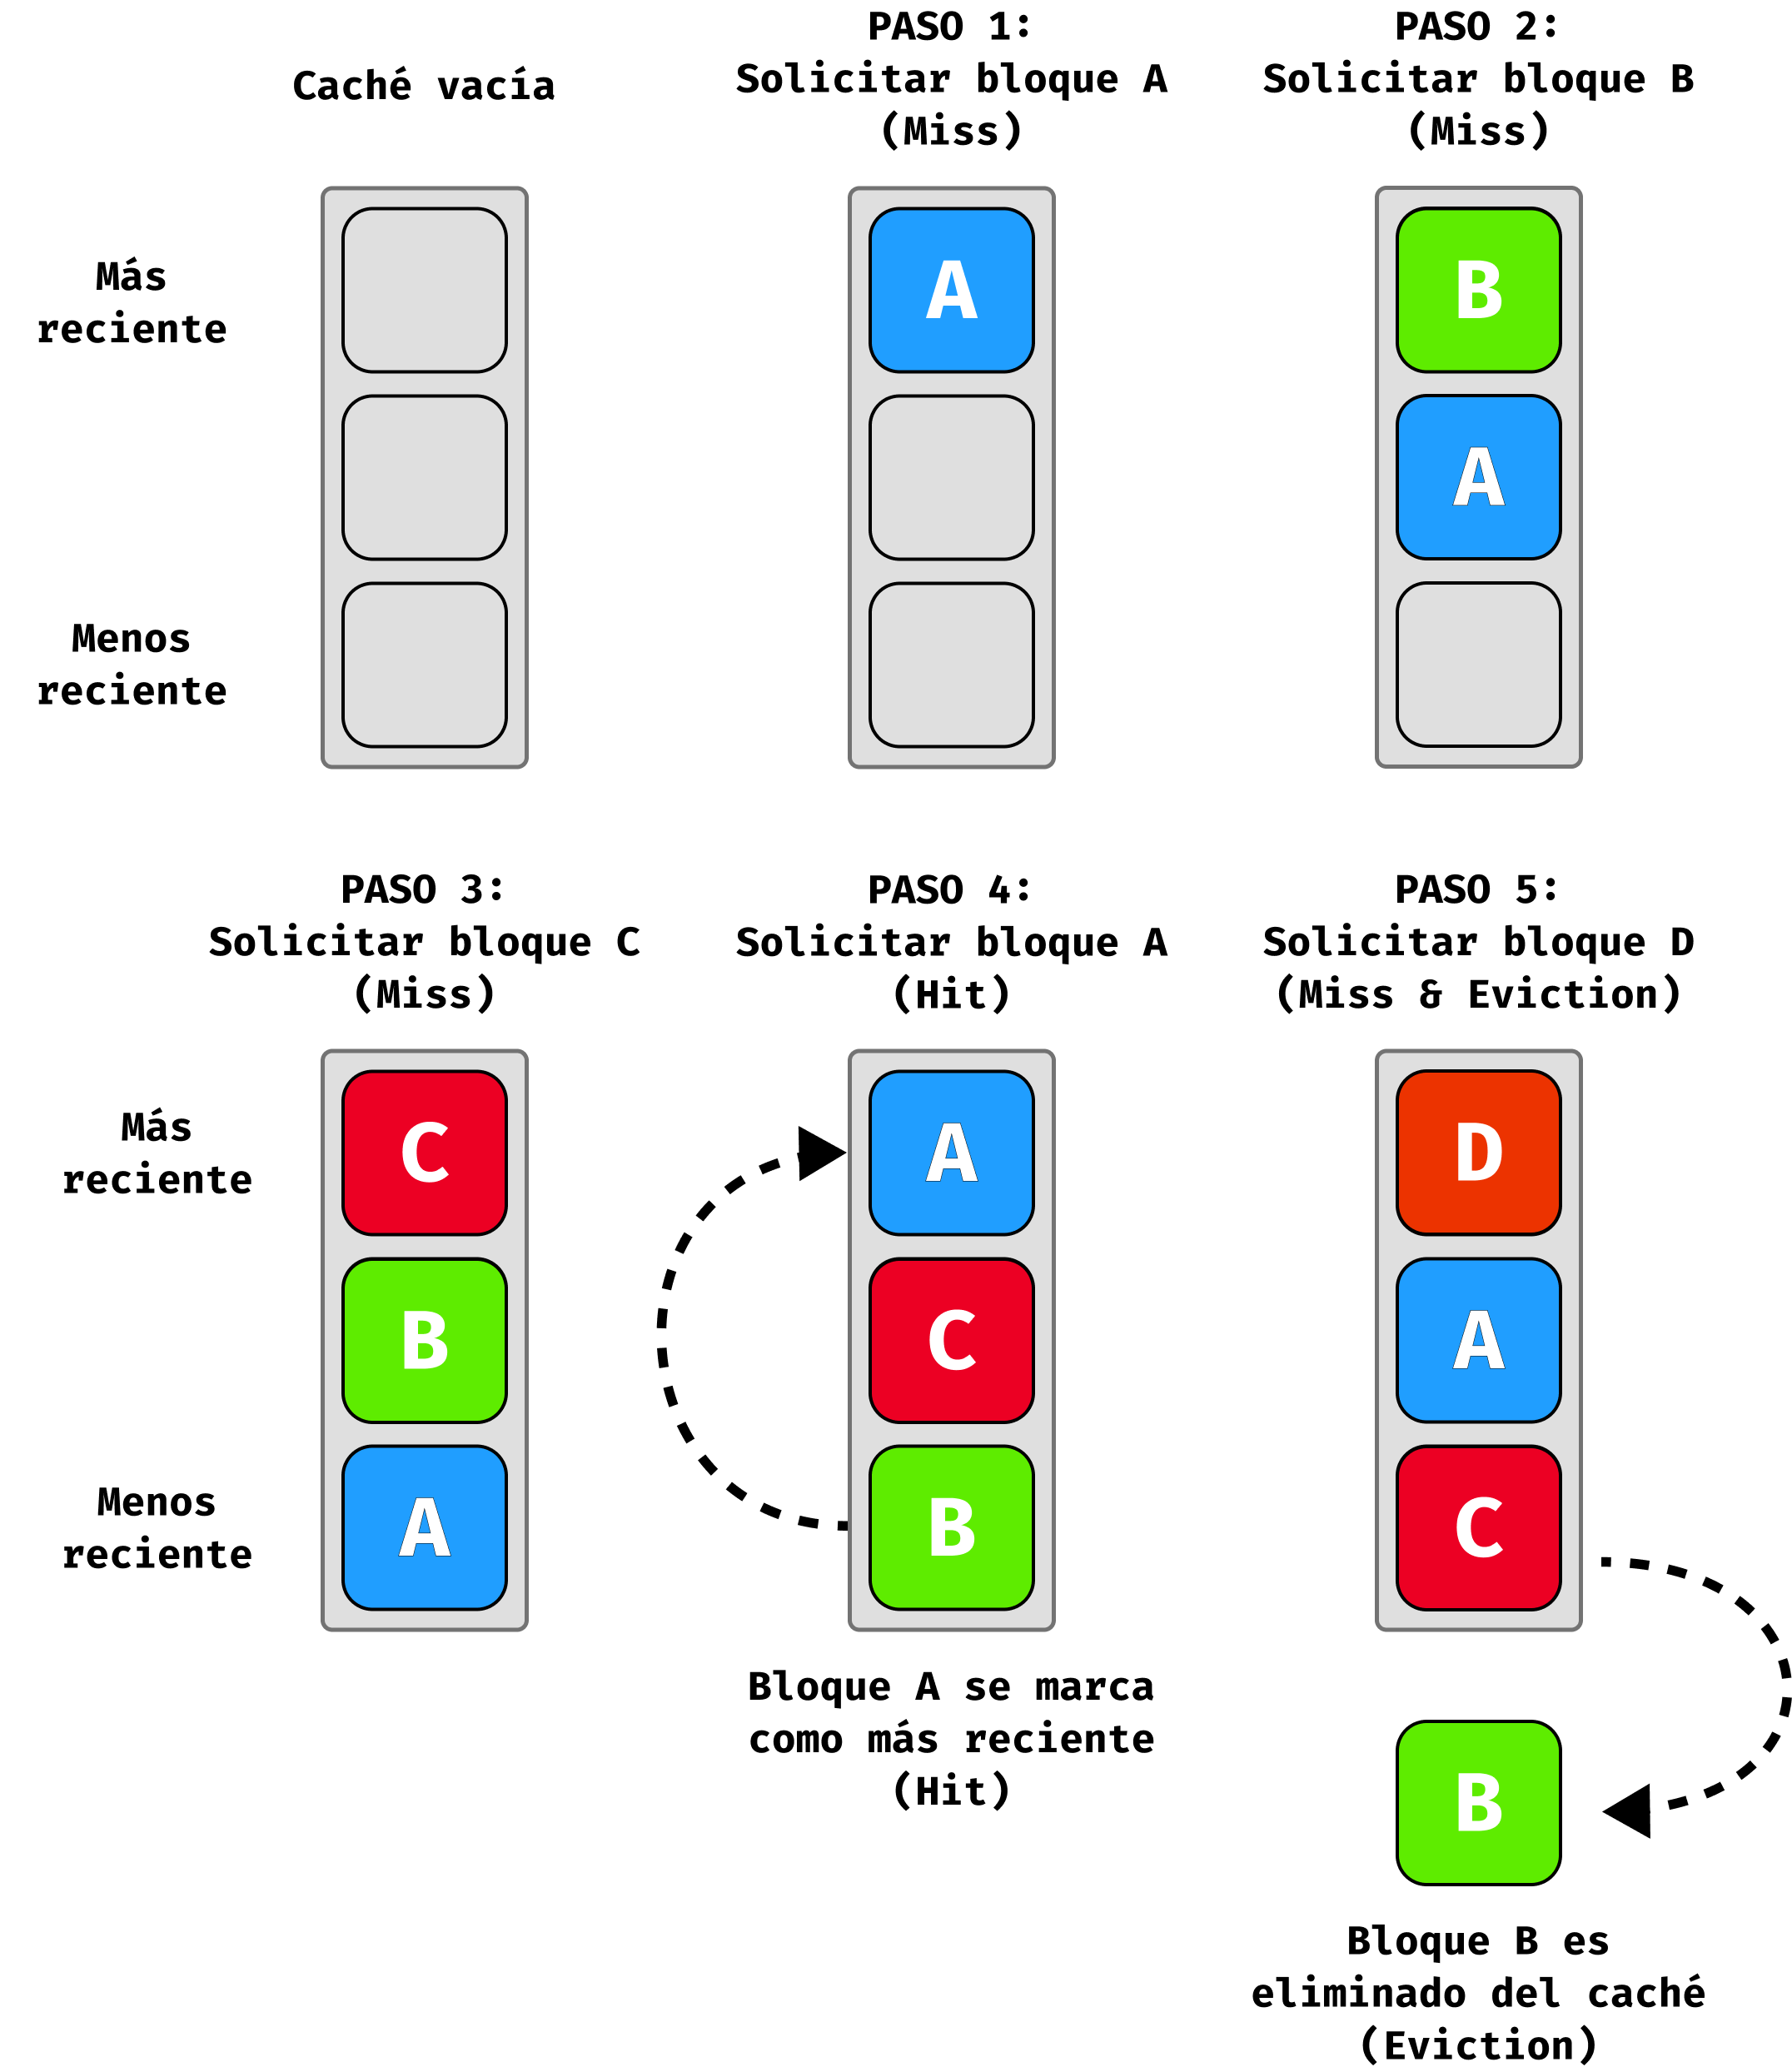
\includegraphics[width=0.6\textwidth]{images/cache-lru.png}
    \label{fig:simulation-design-lru}
\end{figure}
